\section{Documentaci�n autom�tica de este trabajo}
\label{sec:doc-automatica}

La norma IEC 61082 \cite{IEC61082-1:2004} recomienda una serie de
principios para la generaci�n 
autom�tica de documentos sobre electrotecnolog�a.

Las ventajas de este enfoque son muy claras:
\emph{``Cuando la informaci�n es guardada en un formato 
independiente de cualquier presentaci�n, 
esta informaci�n puede ser accesible 
con diferentes vistas y formatos en el momento 
en que sea necesitado y en la forma m�s adecuada 
para los fines previstos.''} \cite{IEC61082-1:2004}

El proceso puede ser observado en la 
figura \ref{fig:Enfoque-documentos-generados-iec61082.eps}. 

\begin{figure}
\begin{center}
  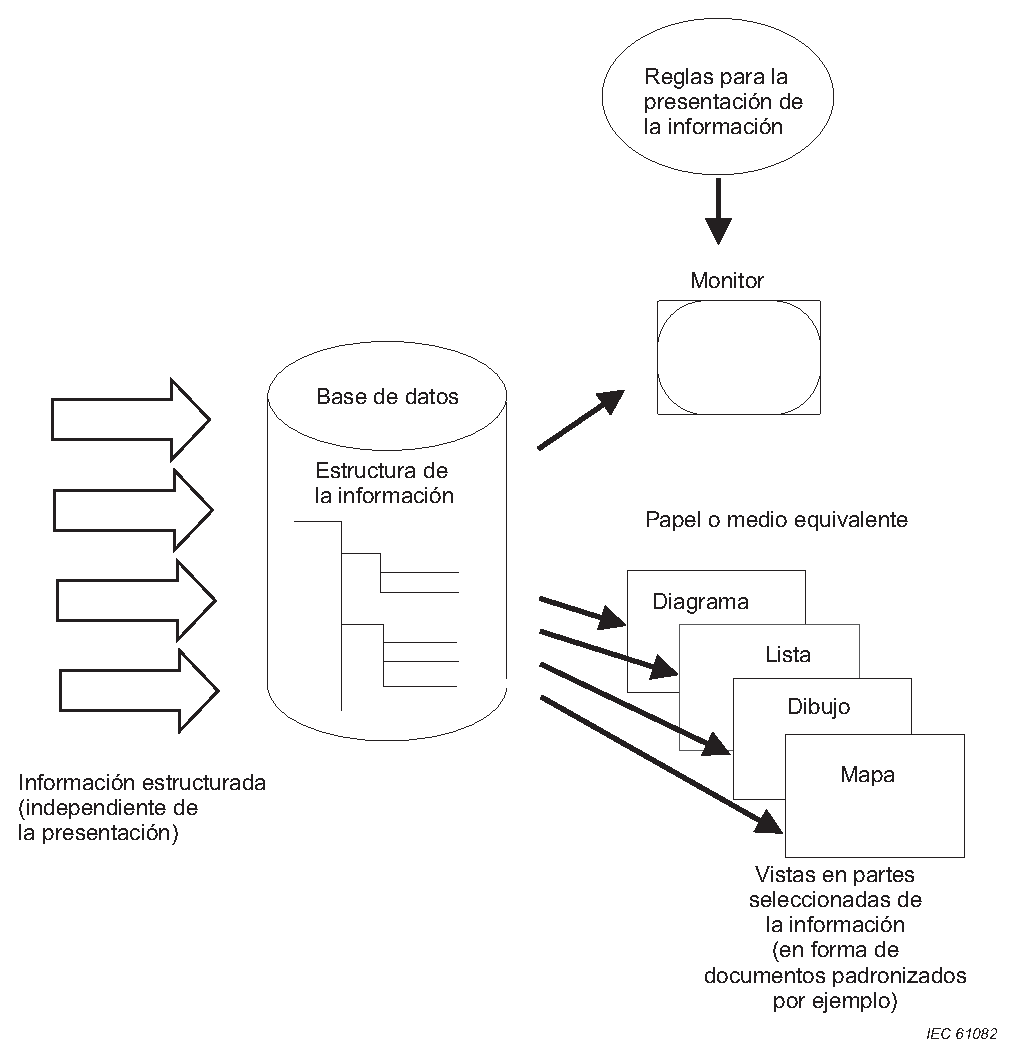
\includegraphics[width=1.0\linewidth]{chapters/enfoque/figures/documentos-generados-iec61082.eps} 
  \caption{Enfoque propuesto por la norma IEC 61802 para la generaci�n de
  documentos sobre electrotecnolog�a} 
  \label{fig:Enfoque-documentos-generados-iec61082.eps}
\end{center}
\end{figure}

Considerando que el \gls{SCL} permite expresar de 
manera formal todo 
el proyecto IEC 61850,
resulta muy sencillo realizar la documentaci�n autom�tica
de este proyecto. Es posible leer los archivos \gls{SCL}
donde se encuentran los modelos de informaci�n
mediante lenguajes de programaci�n que provean librer�as
para la lectura de archivos XML. En este trabajo se ha
utilizado el lenguaje de programaci�n orientado a 
objetos \emph{Python 2.6},
que a partir de los ICDs dise�ados durante
el proceso de ingenier�a,
ha generado en forma autom�tica 
las tablas del cap�tulo \ref{cap:model},
siguiendo las recomendaciones de la norma IEC 61082 \cite{IEC61082-1:2004}

Por lo tanto, de aqu� en m�s, todo el proceso de ingenier�a 
utilizado en este trabajo 
expresa el flujo de trabajo y
los dise�os en t�rminos de \gls{SCL}, 
y los gr�ficos se presentan  
como complemento.



